\documentclass[10pt,a4paper]{article}

\usepackage{graphicx}
\usepackage[left=2cm,right=2cm,top=2cm,bottom=2cm]{geometry}
\usepackage[usenames,dvipsnames,svgnames,table]{xcolor}
\usepackage{placeins}

\newenvironment{ttSection}{\ttfamily}{\par}


\begin{document}

\section{Annotations}

\begin{itemize}
\item \texttt{@NonParadigm(type)} : 'data' or 'active'

\end{itemize}

\section{Analysis Phase}

The current analysis phase takes an SCJ program, compiles it, and analyses it. The output of this section is a list of trees the represent the classes. Since this is SCJ agnostic, we intend to reuse this section. To check this, we have already compiled and analysed a Level~2 program using the current implementation of the tool. The list of trees is used during the translation phase, which we describe next.

\section{Translation}

The major difference between Level~1 and Level~2 programs is the ability to nest mission sequencers and so create a tiered program heirarchy, with clusters of missions and schedulables nested inside other missions. becasue of this key difference, we approach the translation in a heirarchical way. Figure~\ref{fig:translationFlow} shows a flowchart of the translation process. 

\begin{figure}
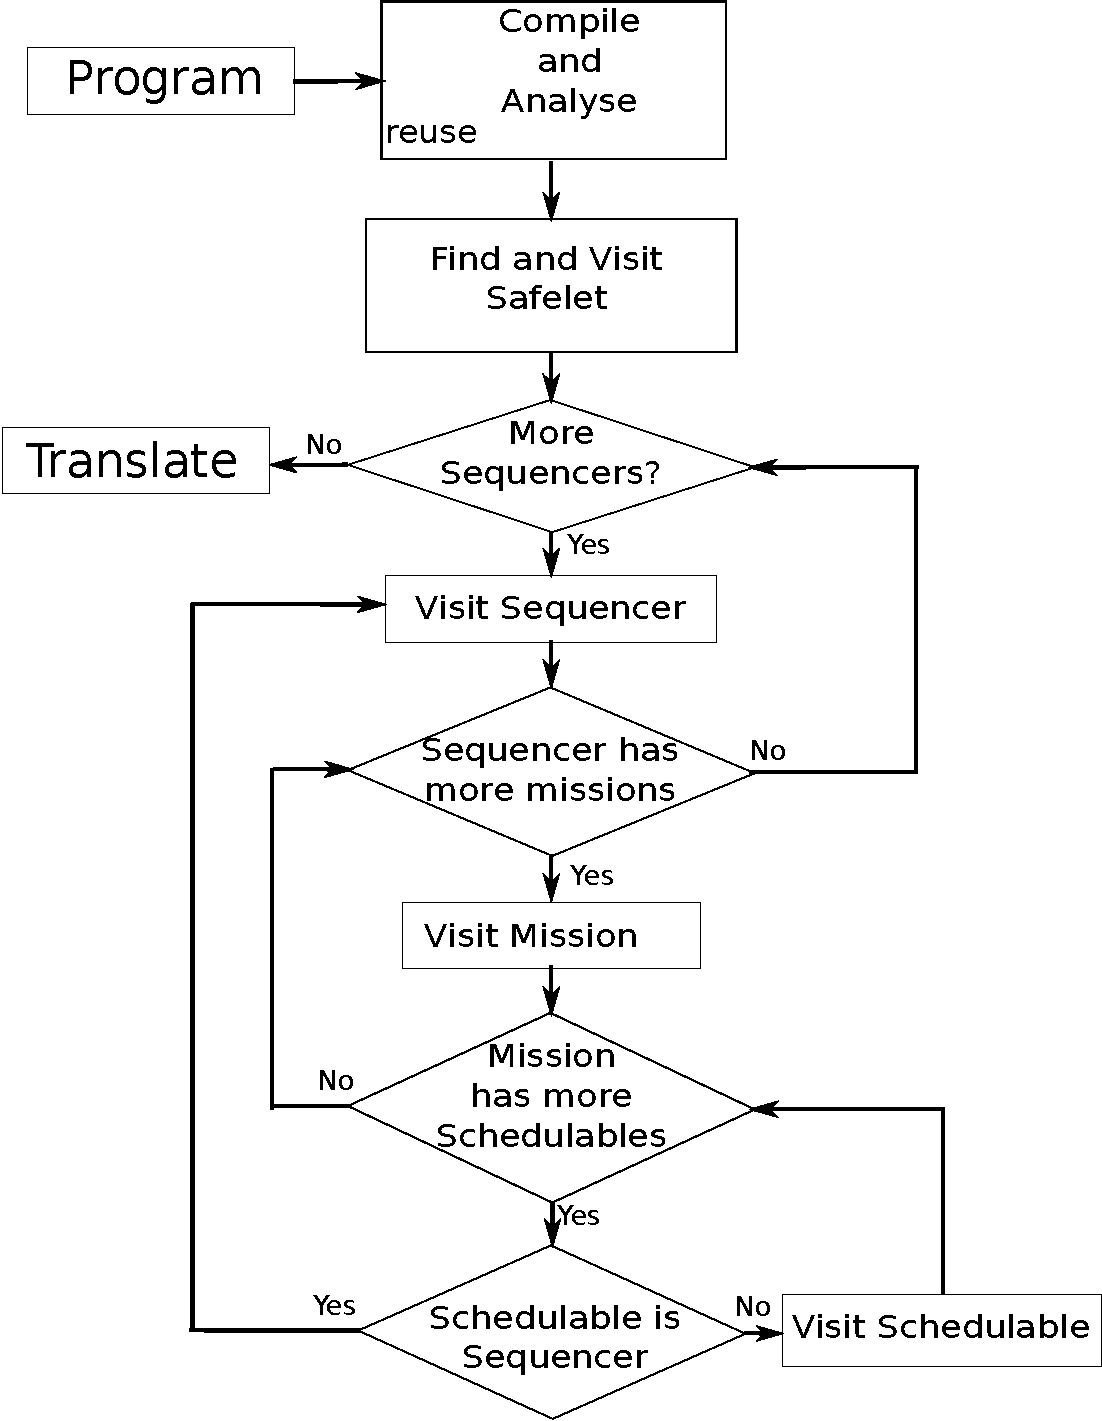
\includegraphics[scale=0.5]{translation.pdf}
\caption{Flowchart of our Translation Process \label{fig:translationFlow} }
\end{figure}

At the top of the diagram we take in the SCJ Program and compile and analyse it, as we describe in the previous section. Then we begin the translation phase. Starting at the top of the program heirarchy, with the safelet, we find the tree belonging to each of the objects within the system. The safelet can be identified easily becasue there is only one in the program. The other objects are identified during the translation process, as we traverse the program's heirarchy, and are explored in that order to ensure that we caputre the heirarchy of the program correctly. beacsue eash class in the program is represented by a tree, we use the visitor pattern to traverse the different types of node that we might find in each tree and extract the information that we need for our translation.

Upon discovery, each object (apart from the safelet) is assigned a unique identifier based upon the class's name. Multiple instances of a class result in multiple identifiers. This identifier is used in our model as a parameter to the processes representing that class. The location of the discovered objects within the program is important for the translation and is recorded.

\subsection{Find and Visit Safelet}

Becasue there is only one safelet in a program, to find the program's safelet we identify the class in the program that implements \texttt{javax.safetycritical.Safelet}.

\begin{ttSection}
Safelet = findSafelet()\\

findSafelet() = \\
for each class in the system, \\
if the class implements javax.safetycritical.Safelet then return it, else continue
\end{ttSection}

Once the safelet is identified we visit it and extract the contents of the \texttt{initializeApplication()} and \texttt{getSequencer()} methods, as well as any program-defined methods. 

The return values of the \texttt{getSequencer()} method are the top-level mission sequencers. The names of the classes that are top-level mission sequencers are collected and used in the next stage of the translation. 

Finally, the name of the safelet class is recorded for use in the translation of the high-level network of the processes in the model.

\subsection{Visit Sequencer}

This translation stage makes use of the top-level sequencer names recorded as the return values from the sfaelet's \texttt{getSequencer()} method. It is also used to translate any nested mission sequencers that are found during the visiting of schedulables. We discus this further in Section~\ref{sec:schedulables}.

We explore all of the missions that a mission sequencer can return and then all of the schedulables that each of its missions can register before moving on to the next mission sequencer. 

When visiting a mission sequencer


\begin{itemize}
\item getNextMission
\end{itemize}

\subsection{Visit Mission}

Each class extends \texttt{javax.safetycritical.Mission} that may be returned by a top-level mission sequencer indicates a cluster in Tier 0. A cluster is a mission and its schedulables. To find the schedulables of a mission we find any class that implements \texttt{javax.safetycritical.ManagedSchedulable} that may be registered during that mission's \texttt{initialize()} method. 

\begin{ttSection}
Tier = a number of Clusters\\

Cluster = Mission and Schedulables
\end{ttSection}

\begin{ttSection}
Schedulables = findSchedulables(mission)\\

findSchedulables(mission) = each class that implements \texttt{javax.safetycritical.ManagedSchedulable} and may be registered in mission.initialize
\end{ttSection}

\begin{itemize}
\item initialize
\item cleanUp
\end{itemize}

\subsection{Visit Schedulable}
\label{sec:schedulables}

If there are one or more schedulables in the tier above that extends \texttt{javax.safetycritical.MissionSequencer} then a nested tier is needed. Nested tiers are composed of clusters in the same way as Tier 0. Each class that extends \texttt{javax.safetycritical.Mission} that may be returned by a mission sequencer in the tier above starts a new cluster. Again, to find the schedulables of a mission we find any class that implements \texttt{javax.safetycritical.ManagedSchedulable} that may be registered during that mission's \texttt{initialize()} method. If any of these schedulables are mission sequencers we begin the process for Nested Tiers again, else we have explored all of the program.

\begin{ttSection}
SchedulableMissionSequencers = findNestedMissionSequencers(Schedulables)\\

findNestedMissionSequencers(schedulables) = \\
for each schedulable in schedulables, \\
if the schedulable extends \texttt{javax.safetycritical.MissionSequencer} then return it, else continue
\end{ttSection}

\begin{ttSection}
Schedulables = findSchedulables(mission)\\

findSchedulables(mission) = each class that implements \texttt{javax.safetycritical.ManagedSchedulable} and may be registered in mission.initialize
\end{ttSection}


\item Handlers
\begin{itemize}
\item handleAsyncEvent
\end{itemize}
\item Managed Thread
\begin{itemize}
\item run
\end{itemize}



































\subsection{Non-Paradigm Objects}

Non-paradigm objects are those objects in the program that do not extend classes or implement interfaces in the SCJ API. During the hierarchical exploration of the program, if any non-paradigm objects are instantiated then they are recorded separately for use in the next phase.



\subsection{Components making Non-paradigm Method Calls}
Because we need to model them differently we must identify when components make non-paradigm method calls. A non-paradigm method call is when a method is called that is not specified in the infrastructure of SCJ, but is program-specific. They can only occur during program-specific code, so we check each method called in application code to see if the class it is declared in is in the SCJ API or not. For methods that are in the SCJ API, they are paradigm method calls. Methods that are declared in the program are non-paradigm method calls. 

\begin{ttSection}
applicationCode = MyClass.getMethodCalls(applicationMethod)\\

For each methodCall in applicationCode, \\
if MyClass.class.getMethod(methodCall).getDeclaredClass() is not javax.safetycritical.Mission \\
then record it as non-paradigm\\
else\\
continue
\end{ttSection}


\subsection{Translate}



The Low-Level Translation takes the set of paradigm object and the set of non-paradigm objects from the analysis. We iterate through these two sets, get the template for the type of object we are dealing with, build the data model for that object, and use the Freemarker template engine to combine these to produce the specification for that object. 

\begin{ttSection}
For each object in ParadigmObjects \\
type = getParadigmObjectType(object) \\
template - getTemplate(type) \\
model = buildDataModel(object,type) \\
combine(model, template)
\end{ttSection}

\begin{ttSection}
For each object in NonParadigmObjects \\
If (isDataObject(object)) \\
template = getDataTemplate()\\
model = buildDataModel(object, 'data')\\
else\\
template = getNonParadigmTemplate() \\
model = buildDataModel(object, 'nonP'

combine(model, template)
\end{ttSection}

\end{document}